% ============================================================================
% CHAPTER 3: FROM BIOLOGICAL TO ARTIFICIAL NEURONS
% ============================================================================

\chapter{From Biological to Artificial Neurons}
\label{ch:neurons}

% ============================================================================
% OVERVIEW
% ============================================================================

\section{Chapter Overview}

This chapter traces the journey from biological neurons---the fundamental units of computation in the brain---to their artificial counterparts that form the foundation of neural networks. We explore the McCulloch-Pitts neuron, the perceptron, and understand both their capabilities and limitations.

\textbf{Learning Objectives:}
\begin{itemize}
    \item Understand the structure and function of biological neurons
    \item Model neurons computationally using the McCulloch-Pitts model
    \item Understand the perceptron with weights and biases
    \item Implement logic gates (AND, OR) using neurons
    \item Recognize the concept of linear separability and its implications
    \item Understand why XOR cannot be solved by a single perceptron
\end{itemize}

% ============================================================================
% BIOLOGICAL NEURONS
% ============================================================================

\section{The Biological Neuron}

\subsection{The Fundamental Unit of Neural Computation}

At the heart of all neural networks lies the \textbf{neuron}---inspired by the biological nerve cells that comprise our brains. The human brain contains approximately 86 billion neurons, interconnected in a vast network that enables thought, memory, and consciousness.

\begin{definitionbox}[Biological Neuron]
A \textbf{biological neuron} (or nerve cell) is the fundamental building block of the brain and nervous system. Neurons transmit information through electrochemical signals.
\end{definitionbox}

\subsection{Structure of a Biological Neuron}

A biological neuron consists of five key components:

\begin{center}
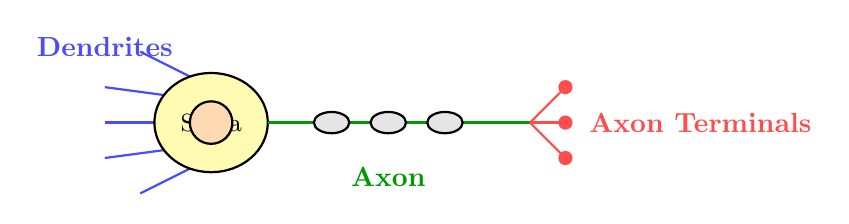
\begin{tikzpicture}[scale=0.9]
    % Dendrites
    \draw[thick, blue!70] (-4,0.5) -- (-2.5,0.3);
    \draw[thick, blue!70] (-4,0) -- (-2.5,0);
    \draw[thick, blue!70] (-4,-0.5) -- (-2.5,-0.3);
    \draw[thick, blue!70] (-3.5,1) -- (-2.5,0.5);
    \draw[thick, blue!70] (-3.5,-1) -- (-2.5,-0.5);
    
    % Cell body (soma)
    \draw[thick, fill=yellow!30] (-2.5,0) ellipse (0.8cm and 0.7cm);
    \node at (-2.5,0) {\small Soma};
    
    % Nucleus
    \draw[thick, fill=orange!30] (-2.5,0) circle (0.3cm);
    
    % Axon
    \draw[thick, green!60!black] (-1.7,0) -- (2,0);
    
    % Myelin sheath bumps
    \foreach \x in {-1,0,1} {
        \draw[thick, fill=gray!20] (\x*0.8,0) ellipse (0.25cm and 0.15cm);
    }
    
    % Axon terminals
    \draw[thick, red!70] (2,0) -- (2.5,0.5);
    \draw[thick, red!70] (2,0) -- (2.5,0);
    \draw[thick, red!70] (2,0) -- (2.5,-0.5);
    \fill[red!70] (2.5,0.5) circle (0.1cm);
    \fill[red!70] (2.5,0) circle (0.1cm);
    \fill[red!70] (2.5,-0.5) circle (0.1cm);
    
    % Labels
    \node[blue!70, above] at (-4,0.8) {\textbf{Dendrites}};
    \node[green!60!black, below] at (0,-0.5) {\textbf{Axon}};
    \node[red!70, right] at (2.7,0) {\textbf{Axon Terminals}};
\end{tikzpicture}
\end{center}

\begin{enumerate}
    \item \textbf{Dendrites}: Branch-like structures that \textit{receive} signals from other neurons. They act as input channels.
    
    \item \textbf{Cell Body (Soma)}: Contains the nucleus and \textit{processes} incoming signals. Integrates all the information received from dendrites.
    
    \item \textbf{Axon}: A long, cable-like structure that \textit{transmits} electrical impulses away from the cell body toward other neurons.
    
    \item \textbf{Axon Terminals}: End points of the axon where signals are passed to other neurons, typically through chemical messengers (neurotransmitters).
    
    \item \textbf{Synapse}: The gap between one neuron's axon terminal and another neuron's dendrite---the site of communication between neurons.
\end{enumerate}

\begin{bluebox}[How Neurons Communicate]
Neurons communicate through two mechanisms:
\begin{enumerate}
    \item \textbf{Electrical signals}: Travel along the axon as action potentials
    \item \textbf{Chemical signals}: Neurotransmitters cross the synaptic gap to trigger the next neuron
\end{enumerate}

When enough input signals arrive at a neuron, it ``fires''---generating an electrical impulse that travels down the axon. This all-or-nothing firing is the basis for neural computation.
\end{bluebox}

% ============================================================================
% ARTIFICIAL NEURONS
% ============================================================================

\section{The Artificial Neuron: Computational Analog}

\subsection{From Biology to Computation}

The key insight that enables artificial neural networks is that we can \textit{abstract} the essential features of biological neurons into a mathematical model:

\begin{center}
\begin{tabular}{|c|c|}
\hline
\textbf{Biological Component} & \textbf{Computational Analog} \\ \hline
Dendrites (receive input) & Input variables $x_1, x_2, \ldots, x_n$ \\ \hline
Signal strength at synapse & Weights $w_1, w_2, \ldots, w_n$ \\ \hline
Cell body (integration) & Summation function $\sum w_i x_i$ \\ \hline
Firing threshold & Activation function $g(\cdot)$ \\ \hline
Axon output & Output $y$ \\ \hline
\end{tabular}
\end{center}

\subsection{General Structure of an Artificial Neuron}

\begin{center}
\begin{tikzpicture}[
    node/.style={circle, draw, minimum size=1cm},
    input/.style={circle, draw, fill=blue!20, minimum size=0.8cm},
    output/.style={circle, draw, fill=red!20, minimum size=0.8cm}
]
    % Input nodes
    \node[input] (x1) at (-3, 1.5) {$x_1$};
    \node[input] (x2) at (-3, 0) {$x_2$};
    \node[input] (x3) at (-3, -1.5) {$x_n$};
    \node at (-3, -0.75) {$\vdots$};
    
    % Aggregation
    \node[draw, rounded corners, minimum width=1.5cm, minimum height=2cm, fill=yellow!20] (agg) at (0, 0) {};
    \node at (0, 0.5) {$\sum$};
    \node at (0, -0.3) {\small$g(\cdot)$};
    
    % Output
    \node[output] (y) at (3, 0) {$y$};
    
    % Connections with weights
    \draw[-Stealth] (x1) -- node[above, sloped] {\small$w_1$} (agg);
    \draw[-Stealth] (x2) -- node[above, sloped] {\small$w_2$} (agg);
    \draw[-Stealth] (x3) -- node[above, sloped] {\small$w_n$} (agg);
    
    % Output connection
    \draw[-Stealth, thick] (agg) -- (y);
    
    % Labels
    \node[below=0.5cm] at (-3,-2) {Inputs};
    \node[below=0.5cm] at (0,-2) {Aggregation \& Activation};
    \node[below=0.5cm] at (3,-2) {Output};
\end{tikzpicture}
\end{center}

The artificial neuron performs two operations:
\begin{enumerate}
    \item \textbf{Aggregation}: Compute weighted sum of inputs: $z = \sum_{i=1}^{n} w_i x_i$
    \item \textbf{Activation}: Apply a decision function: $y = g(z)$
\end{enumerate}

% ============================================================================
% MCCULLOCH-PITTS NEURON
% ============================================================================

\section{The McCulloch-Pitts Neuron (1943)}

\subsection{The First Computational Neuron Model}

In 1943, Warren McCulloch (neuroscientist) and Walter Pitts (logician) proposed the first mathematical model of a neuron. This model laid the groundwork for all subsequent neural network research.

\begin{definitionbox}[McCulloch-Pitts (MP) Neuron]
The MP neuron has the following characteristics:
\begin{itemize}
    \item \textbf{Inputs}: Binary values $x_i \in \{0, 1\}$
    \item \textbf{Weights}: All equal to 1 (uniform weighting)
    \item \textbf{Aggregation}: Simple summation $\sum_{i=1}^{n} x_i$
    \item \textbf{Activation}: Threshold function
\end{itemize}

The neuron fires (outputs 1) if and only if:
\[
\sum_{i=1}^{n} x_i \geq \theta
\]
where $\theta$ is the threshold.
\end{definitionbox}

\subsection{Thresholding Logic}

The activation function in MP neurons is a \textbf{step function}:

\[
y = g\left(\sum_{i=1}^{n} x_i\right) = 
\begin{cases}
1 & \text{if } \sum_{i=1}^{n} x_i \geq \theta \\
0 & \text{otherwise}
\end{cases}
\]

\begin{center}
\begin{tikzpicture}
    \draw[->] (-2,0) -- (3,0) node[right] {$\sum x_i$};
    \draw[->] (0,-0.5) -- (0,2) node[above] {$y$};
    
    \draw[very thick, blue] (-2,0) -- (1,0);
    \draw[very thick, blue] (1,1.5) -- (3,1.5);
    \draw[thick, blue, dashed] (1,0) -- (1,1.5);
    
    \node[below] at (1,0) {$\theta$};
    \node[left] at (0,1.5) {$1$};
    \fill[blue] (1,1.5) circle (2pt);
    \draw[blue, fill=white] (1,0) circle (2pt);
\end{tikzpicture}
\end{center}

\subsection{Inhibitory and Excitatory Inputs}

McCulloch and Pitts recognized that biological neurons have two types of inputs:

\begin{itemize}
    \item \textbf{Excitatory inputs}: Contribute positively toward reaching the threshold. They ``encourage'' the neuron to fire.
    
    \item \textbf{Inhibitory inputs}: Block the neuron from firing regardless of other inputs. If an inhibitory input is active, the neuron outputs 0.
\end{itemize}

\begin{examplebox}[Decision Example]
Should I go to college today?

Inputs:
\begin{itemize}
    \item $x_1$: Is my friend going? (excitatory)
    \item $x_2$: Is the weather nice? (excitatory)
    \item $x_3$: Do I have an exam? (excitatory)
    \item $x_4$: Am I seriously ill? (inhibitory)
\end{itemize}

If $x_4 = 1$ (ill), the output is 0 regardless of other inputs.
Otherwise, if $x_1 + x_2 + x_3 \geq 2$, go to college.
\end{examplebox}

% ============================================================================
% LOGIC GATES WITH NEURONS
% ============================================================================

\section{Implementing Logic Gates}

\subsection{The Computational Foundation}

Digital computers perform all computations using logic gates. If neurons can implement logic gates, they can potentially compute any function!

\subsection{OR Gate}

\begin{minipage}{0.45\textwidth}
\textbf{Truth Table:}
\begin{center}
\begin{tabular}{|c|c|c|}
\hline
$x_1$ & $x_2$ & OR \\ \hline
0 & 0 & 0 \\ \hline
0 & 1 & 1 \\ \hline
1 & 0 & 1 \\ \hline
1 & 1 & 1 \\ \hline
\end{tabular}
\end{center}
\end{minipage}
\hfill
\begin{minipage}{0.45\textwidth}
\textbf{Implementation:}
\[
\text{Threshold: } \theta = 1
\]
\[
y = \begin{cases} 1 & \text{if } x_1 + x_2 \geq 1 \\ 0 & \text{otherwise} \end{cases}
\]
\end{minipage}

\subsection{AND Gate}

\begin{minipage}{0.45\textwidth}
\textbf{Truth Table:}
\begin{center}
\begin{tabular}{|c|c|c|}
\hline
$x_1$ & $x_2$ & AND \\ \hline
0 & 0 & 0 \\ \hline
0 & 1 & 0 \\ \hline
1 & 0 & 0 \\ \hline
1 & 1 & 1 \\ \hline
\end{tabular}
\end{center}
\end{minipage}
\hfill
\begin{minipage}{0.45\textwidth}
\textbf{Implementation:}
\[
\text{Threshold: } \theta = 2
\]
\[
y = \begin{cases} 1 & \text{if } x_1 + x_2 \geq 2 \\ 0 & \text{otherwise} \end{cases}
\]
\end{minipage}

\subsection{NOT Gate}

Using an inhibitory input:
\[
y = \begin{cases} 1 & \text{if } x = 0 \\ 0 & \text{if } x = 1 \end{cases}
\]

% ============================================================================
% LINEAR SEPARABILITY
% ============================================================================

\section{Geometric Interpretation: Linear Separability}

\subsection{Decision Boundaries}

When we set a threshold condition like $x_1 + x_2 \geq \theta$, we're defining a \textbf{linear decision boundary} in the input space.

\begin{center}
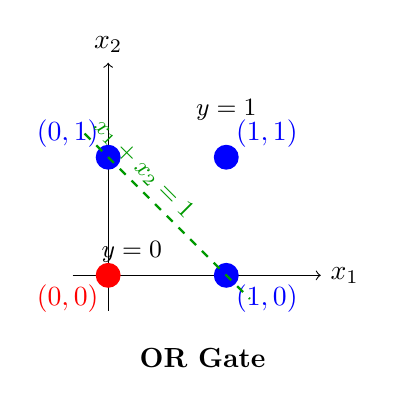
\begin{tikzpicture}[scale=1.5]
    % Axes
    \draw[->] (-0.3,0) -- (1.8,0) node[right] {$x_1$};
    \draw[->] (0,-0.3) -- (0,1.8) node[above] {$x_2$};
    
    % Grid points
    \fill[red] (0,0) circle (3pt) node[below left] {$(0,0)$};
    \fill[blue] (0,1) circle (3pt) node[above left] {$(0,1)$};
    \fill[blue] (1,0) circle (3pt) node[below right] {$(1,0)$};
    \fill[blue] (1,1) circle (3pt) node[above right] {$(1,1)$};
    
    % Decision boundary
    \draw[thick, green!60!black, dashed] (-0.2,1.2) -- (1.2,-0.2);
    
    % Labels
    \node[green!60!black, rotate=-45] at (0.3,0.9) {\small$x_1 + x_2 = 1$};
    
    % Regions
    \node at (0.2,0.2) {\small$y=0$};
    \node at (1,1.4) {\small$y=1$};
    
    \node at (0.8,-0.7) {\textbf{OR Gate}};
\end{tikzpicture}
\hspace{1cm}
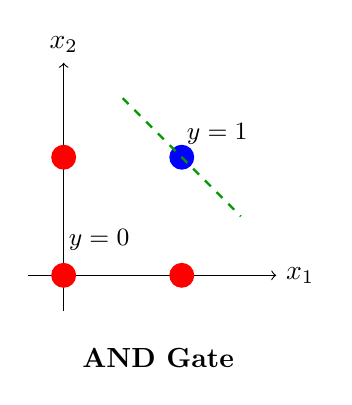
\begin{tikzpicture}[scale=1.5]
    % Axes
    \draw[->] (-0.3,0) -- (1.8,0) node[right] {$x_1$};
    \draw[->] (0,-0.3) -- (0,1.8) node[above] {$x_2$};
    
    % Grid points
    \fill[red] (0,0) circle (3pt);
    \fill[red] (0,1) circle (3pt);
    \fill[red] (1,0) circle (3pt);
    \fill[blue] (1,1) circle (3pt);
    
    % Decision boundary
    \draw[thick, green!60!black, dashed] (0.5,1.5) -- (1.5,0.5);
    
    % Regions
    \node at (0.3,0.3) {\small$y=0$};
    \node at (1.3,1.2) {\small$y=1$};
    
    \node at (0.8,-0.7) {\textbf{AND Gate}};
\end{tikzpicture}
\end{center}

\begin{definitionbox}[Linear Separability]
A dataset is \textbf{linearly separable} if there exists a hyperplane (a line in 2D, a plane in 3D) that perfectly separates the classes.

Mathematically, data points $\{(\vect{x}_i, y_i)\}$ are linearly separable if there exist weights $\vect{w}$ and bias $b$ such that:
\[
\vect{w}^\top \vect{x}_i + b > 0 \text{ for all } y_i = 1
\]
\[
\vect{w}^\top \vect{x}_i + b < 0 \text{ for all } y_i = 0
\]
\end{definitionbox}

\subsection{The XOR Problem}

Consider the XOR (exclusive OR) function:

\begin{center}
\begin{tabular}{|c|c|c|}
\hline
$x_1$ & $x_2$ & XOR \\ \hline
0 & 0 & \textcolor{red}{0} \\ \hline
0 & 1 & \textcolor{blue}{1} \\ \hline
1 & 0 & \textcolor{blue}{1} \\ \hline
1 & 1 & \textcolor{red}{0} \\ \hline
\end{tabular}
\end{center}

\begin{center}
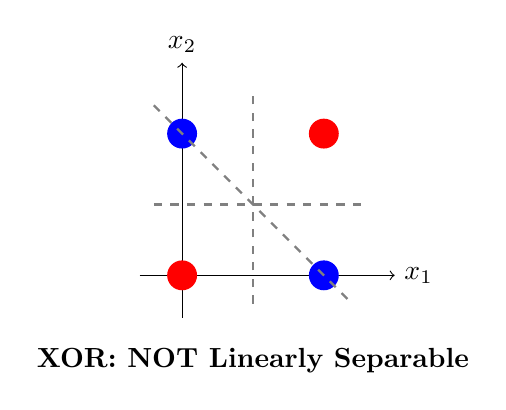
\begin{tikzpicture}[scale=1.8]
    % Axes
    \draw[->] (-0.3,0) -- (1.5,0) node[right] {$x_1$};
    \draw[->] (0,-0.3) -- (0,1.5) node[above] {$x_2$};
    
    % Grid points
    \fill[red] (0,0) circle (3pt);
    \fill[blue] (0,1) circle (3pt);
    \fill[blue] (1,0) circle (3pt);
    \fill[red] (1,1) circle (3pt);
    
    % Attempted lines (showing impossibility)
    \draw[thick, gray, dashed] (-0.2,0.5) -- (1.3,0.5);
    \draw[thick, gray, dashed] (0.5,-0.2) -- (0.5,1.3);
    \draw[thick, gray, dashed] (-0.2,1.2) -- (1.2,-0.2);
    
    \node at (0.5,-0.6) {\textbf{XOR: NOT Linearly Separable}};
\end{tikzpicture}
\end{center}

\begin{importantbox}[The XOR Problem]
\textbf{No single line can separate the blue points from the red points.}

This means a single MP neuron (or a single perceptron) \textbf{cannot} compute the XOR function. This limitation, famously pointed out by Minsky and Papert (1969), temporarily halted neural network research.

The solution: \textbf{multiple layers} of neurons!
\end{importantbox}

% ============================================================================
% THE PERCEPTRON
% ============================================================================

\section{The Perceptron (1958)}

\subsection{Addressing MP Neuron Limitations}

Frank Rosenblatt introduced the \textbf{perceptron} in 1958 to address three limitations of the MP neuron:

\begin{enumerate}
    \item \textbf{Binary inputs only} $\rightarrow$ Allow real-valued inputs
    \item \textbf{Equal weights} $\rightarrow$ Allow learnable weights
    \item \textbf{Fixed threshold} $\rightarrow$ Replace with learnable bias
\end{enumerate}

\begin{definitionbox}[The Perceptron]
The perceptron computes:
\[
y = g\left(\sum_{i=1}^{n} w_i x_i + b\right) = g(\vect{w}^\top \vect{x} + b)
\]
where:
\begin{itemize}
    \item $x_i \in \R$: Real-valued inputs
    \item $w_i \in \R$: Learnable weights
    \item $b \in \R$: Learnable bias
    \item $g(\cdot)$: Step activation function
\end{itemize}
\[
g(z) = \begin{cases} 1 & \text{if } z \geq 0 \\ 0 & \text{otherwise} \end{cases}
\]
\end{definitionbox}

\subsection{Understanding the Bias Term}

The bias $b$ serves as a learnable threshold. It controls how ``eager'' the neuron is to fire:

\begin{itemize}
    \item \textbf{Positive bias}: Neuron tends to fire (biased toward positive output)
    \item \textbf{Negative bias}: Neuron is reluctant to fire (biased toward negative output)
\end{itemize}

\begin{bluebox}[Bias as Built-in Preference]
Think of bias as the neuron's ``default tendency.'' 

Example: A neuron deciding whether to go to college:
\begin{itemize}
    \item If you love college: High positive bias (you'll go unless many factors are negative)
    \item If you dislike college: Negative bias (you need many positive factors to go)
\end{itemize}
\end{bluebox}

\subsection{Parameters: What the Perceptron Learns}

\begin{center}
\begin{tabular}{|c|c|c|}
\hline
\textbf{Component} & \textbf{Symbol} & \textbf{Type} \\ \hline
Inputs & $x_1, \ldots, x_n$ & Fixed (given) \\ \hline
Weights & $w_1, \ldots, w_n$ & Learnable \\ \hline
Bias & $b$ & Learnable \\ \hline
Output & $y$ & Computed \\ \hline
\end{tabular}
\end{center}

\textbf{Learning} = Finding the right values for weights and bias from data.

% ============================================================================
% PERCEPTRON LEARNING
% ============================================================================

\section{The Perceptron Learning Algorithm}

\subsection{Learning from Data}

Instead of manually setting weights, we want to \textbf{learn} them from labeled examples. Given training data $\{(\vect{x}_i, y_i)\}$, find $\vect{w}$ and $b$ such that the perceptron correctly classifies all examples.

\subsection{The Algorithm}

\begin{enumerate}
    \item \textbf{Initialize} weights $\vect{w}$ and bias $b$ (e.g., to zeros or small random values)
    \item \textbf{For each} training example $(\vect{x}, y)$:
    \begin{enumerate}
        \item Compute prediction: $\hat{y} = g(\vect{w}^\top \vect{x} + b)$
        \item If $\hat{y} \neq y$ (misclassification):
        \[
        \vect{w} \leftarrow \vect{w} + (y - \hat{y}) \vect{x}
        \]
        \[
        b \leftarrow b + (y - \hat{y})
        \]
    \end{enumerate}
    \item \textbf{Repeat} until all examples are correctly classified (or max iterations)
\end{enumerate}

\begin{bluebox}[Intuition Behind the Update Rule]
\begin{itemize}
    \item If $y = 1$ but $\hat{y} = 0$ (false negative):
    \begin{itemize}
        \item We need to increase $\vect{w}^\top \vect{x} + b$
        \item Update: $\vect{w} \leftarrow \vect{w} + \vect{x}$ (add the input to weights)
    \end{itemize}
    \item If $y = 0$ but $\hat{y} = 1$ (false positive):
    \begin{itemize}
        \item We need to decrease $\vect{w}^\top \vect{x} + b$
        \item Update: $\vect{w} \leftarrow \vect{w} - \vect{x}$ (subtract the input)
    \end{itemize}
\end{itemize}
\end{bluebox}

\subsection{Convergence Theorem}

\begin{theorembox}[Perceptron Convergence Theorem]
If the training data is \textbf{linearly separable}, the perceptron learning algorithm will converge to a solution (find separating weights) in a \textbf{finite number of steps}.
\end{theorembox}

This is both good and bad news:
\begin{itemize}
    \item \textbf{Good}: Guaranteed to find a solution if one exists
    \item \textbf{Bad}: If data is not linearly separable, the algorithm never converges
\end{itemize}

% ============================================================================
% PYTHON IMPLEMENTATION
% ============================================================================

\section{Python Implementation of the Perceptron}

Now that we have established the theoretical foundation of the perceptron learning algorithm, let us implement it from scratch in Python.

\subsection{Visualizing Error Surfaces}

During training, we are trying to find the optimal weights $\vect{w}$ and bias $b$ that minimize our classification error. We can visualize this as searching for the lowest point on an \textbf{error surface}. Every point on this surface corresponds to a specific combination of weights and bias, and the height represents the number of misclassified points (the error).

\subsection{The Code}

\begin{lstlisting}[language=Python, caption={Perceptron Training Algorithm}]
import numpy as np

def train_perceptron(X, y, max_iters=1000):
    """
    Trains a perceptron using the perceptron learning algorithm.
    X: Inputs (N x d) setup for the linearly separable problem
    y: Labels (N), where 1 is positive class, 0 is negative class
    """
    n_samples, n_features = X.shape
    
    # Step 1: Initialize weights randomly
    w = np.random.randn(n_features)
    
    for step in range(max_iters):
        misclassified = False
        
        # Step 2: Loop through data points randomly
        # Permute points to avoid cyclic toggling
        indices = np.random.permutation(n_samples)
        
        for i in indices:
            xi = X[i]
            label = y[i]
            
            # Predict
            dot_product = np.dot(w, xi)
            prediction = 1 if dot_product >= 0 else 0
            
            # Step 3: Check for misclassification and update weights
            if prediction != label:
                misclassified = True
                
                # Rule: w = w + (2y - 1) * xi
                # If label is 1, pred is 0 -> add xi
                # If label is 0, pred is 1 -> subtract xi
                w += (2 * label - 1) * xi
                
        # Step 4: Check if converged
        if not misclassified:
            print(f"Converged at step {step}")
            break
            
    return w
\end{lstlisting}

In this algorithm, the `misclassified` flag checks whether any point was wrongly labeled during an epoch. If the data is linearly separable, the algorithm finishes in a finite number of iterations when `misclassified` remains \texttt{False} for the entire loop.

% ============================================================================
% MULTICLASS CLASSIFICATION
% ============================================================================

\section{Multiclass Classification}

The perceptron, as developed by Rosenblatt, is intrinsically a \textbf{binary classifier}. It draws a single hyperplane dividing the $n$-dimensional space into two half-spaces (e.g., $y=1$ and $y=0$). What do we do when our dataset contains more than two classes (e.g., distinguishing between 10 different digits)?

To adapt a binary classifier for a multiclass problem, we use the \textbf{One-Versus-All} (or One-Versus-Rest) technique. 

\begin{enumerate}
    \item Assume we have $K$ classes (e.g., 1 to 10).
    \item We train $K$ separate binary perceptrons. 
    \item The first perceptron is trained to distinguish Class 1 against all other classes (Classes 2 through 10).
    \item The second perceptron distinguishes Class 2 against the rest.
    \item This process is repeated until we have a distinct binary classifier trained for each unique class.
\end{enumerate}

During prediction, when given a new input point, we pass it through all $K$ perceptrons. The final predicted class is the one associated with the perceptron that fires with the greatest confidence.

% ============================================================================
% PERCEPTRON CONVERGENCE THEOREM FORMULATION
% ============================================================================

\section{Formulating the Proof of Convergence}

We stated earlier that if the dataset is linearly separable, the perceptron is guaranteed to converge. But without a mathematical proof, there is a risk that the algorithm could toggle endlessly. For instance, adjusting weights to fix an error on point $A$ might inadvertently misclassify point $B$, and adjusting to fix point $B$ misclassifies point $A$ again.

To formally prevent this toggling concern, we must formulate the theorem mathematically. We define the premise as follows:

\begin{theorembox}[Premise for Convergence Proof]
Let $\mathcal{P}, \mathcal{N} \subset \R^n$ be two finite sets of points defining our positive and negative classes. Assume $\mathcal{P}$ and $\mathcal{N}$ are \textbf{linearly separable}, meaning there exists some optimal weight vector $\vect{w}^*$ such that:
\begin{align*}
    (\vect{w}^*)^\top \vect{x} &> 0 \quad \text{for all } \vect{x} \in \mathcal{P} \\
    (\vect{w}^*)^\top \vect{x} &< 0 \quad \text{for all } \vect{x} \in \mathcal{N}
\end{align*}
Under this premise, the perceptron learning algorithm converges in a finite number of update steps.
\end{theorembox}

The rigorous proof of this theorem requires demonstrating that each update step inevitably brings the current weight vector $\vect{w}$ closer to the optimal solution $\vect{w}^*$, by monitoring their cosine angle (the dot product relative to their magnitudes). This proof mechanism establishes confidence that simple perceptron learning functions without entering infinite loops.

% ============================================================================
% SUMMARY
% ============================================================================

\section{Chapter Summary}

\begin{itemize}
    \item \textbf{Biological neurons} are the brain's computational units, composed of dendrites (input), soma (processing), axon (transmission), and synapses (communication).
    
    \item \textbf{Artificial neurons} abstract biological neurons into mathematical models with inputs, weights, aggregation (summation), and activation (threshold).
    
    \item The \textbf{McCulloch-Pitts neuron} (1943) uses binary inputs, uniform weights, and thresholding logic. It can implement AND, OR, and NOT gates.
    
    \item \textbf{Linear separability}: A single neuron can only solve problems where classes can be separated by a hyperplane.
    
    \item The \textbf{XOR problem}: XOR is not linearly separable, so a single neuron cannot solve it. This motivates multi-layer networks.
    
    \item The \textbf{perceptron} (1958) adds real-valued inputs, learnable weights, and learnable bias, making learning from data possible.
    
    \item \textbf{Learning in neural networks} = adjusting weights and biases to minimize errors on training data.
\end{itemize}

\begin{bluebox}[Looking Ahead]
The limitations of single neurons (especially the XOR problem) lead us toward:
\begin{enumerate}
    \item \textbf{Multi-layer networks}: Stacking neurons to solve non-linearly separable problems
    \item \textbf{Smooth activation functions}: Replacing the step function with differentiable functions like sigmoid, enabling gradient-based learning
    \item \textbf{Backpropagation}: An algorithm to efficiently compute how to adjust weights in deep networks
\end{enumerate}
\end{bluebox}
